\documentclass[11pt]{article}
\usepackage[T1]{fontenc}
\usepackage{lmodern}
\usepackage[a4paper,left=25mm,right=30mm,top=22mm,bottom=24mm,marginparwidth=18mm]{geometry}
\usepackage{amsmath,amssymb,mathtools,stmaryrd}
\usepackage{tikz}
\usetikzlibrary{arrows.meta,calc,positioning}
\usepackage{caption}
\usepackage{xcolor}
\usepackage{marginnote}
\usepackage{microtype}
\usepackage{needspace}
\usepackage[hidelinks]{hyperref}
\definecolor{LeanTeal}{HTML}{087F72}
\definecolor{SourceGray}{HTML}{66736F}
\setlength{\parindent}{0pt}
\setlength{\parskip}{0.55em}
\setlength{\emergencystretch}{2em}
\newcommand{\leanmarker}[2]{%
  \Needspace{3\baselineskip}%
  \marginnote{\hyperlink{#1}{\color{LeanTeal}\fbox{\scriptsize Lean}}}%
  \hypertarget{#1}{\textbf{#2.}}%
}
\newcommand{\sourcepage}[1]{\par\medskip\noindent\textcolor{SourceGray}{\scriptsize Source PDF page #1}\par\smallskip}
\pagestyle{plain}
\begin{document}
\begin{center}\LARGE\bfseries Equational theories\par\medskip
\large Lean 4 Formalization Companion -- Chapter 6\end{center}
\medskip
\noindent\textit{This project-generated reading copy contains reviewed mathematical items, short source locators, and redrawn diagrams. It does not reproduce the original PDF or automatic OCR prose. Click a Lean tag in the web reader to open the mapped Lean declaration.}
\bigskip\hrule\bigskip
\section*{Section 6.1}
\sourcepage{86}
\leanmarker{prop-6-1-1}{Proposition 6.1.1} Dcpo algebras form a complete category.

\leanmarker{thm-6-1-2}{Theorem 6.1.2} Free dcpo algebras exist for inequational theories.

\begin{center}
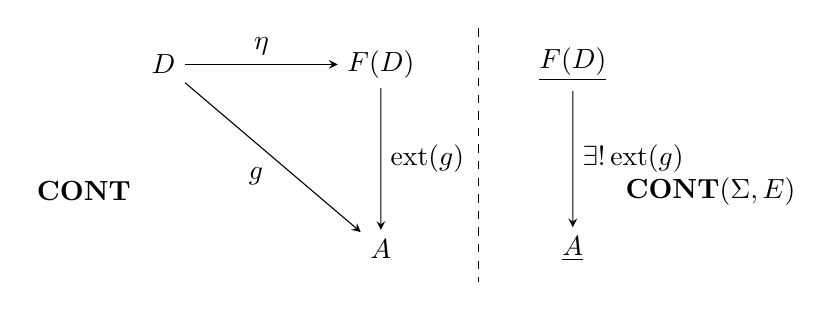
\begin{tikzpicture}[scale=0.92, >=stealth]
  \node (D)  at (0,1.65) {$D$};
  \node (FD) at (3.0,1.65) {$F(D)$};
  \node (A)  at (3.0,-0.9) {$A$};
  \draw[->] (D) -- node[above] {$\eta$} (FD);
  \draw[->] (D) -- node[below left] {$g$} (A);
  \draw[->] (FD) -- node[right] {$\operatorname{ext}(g)$} (A);
  \node[font=\bfseries] at (-1.1,-0.1) {CONT};
  \draw[dashed] (4.35,2.15) -- (4.35,-1.35);
  \node (FDa) at (5.65,1.65) {$\underline{F(D)}$};
  \node (Aa)  at (5.65,-0.9) {$\underline{A}$};
  \draw[->] (FDa) -- node[right] {$\exists!\operatorname{ext}(g)$} (Aa);
  \node[font=\bfseries] at (7.55,-0.1) {CONT$(\Sigma,E)$};
\end{tikzpicture}
\end{center}

\[
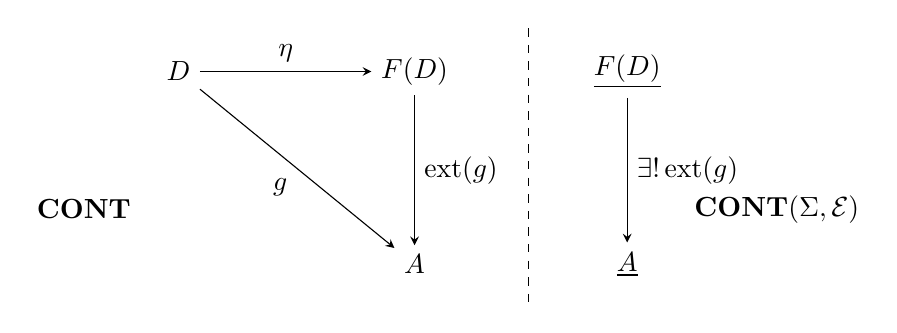
\begin{tikzpicture}[baseline=(current bounding box.center), >=stealth]
  \node (D)  at (0,1.5) {$D$};
  \node (FD) at (3.0,1.5) {$F(D)$};
  \node (A)  at (3.0,-0.95) {$A$};
  \draw[->] (D) -- node[above] {$\eta$} (FD);
  \draw[->] (D) -- node[below left] {$g$} (A);
  \draw[->] (FD) -- node[right] {$\operatorname{ext}(g)$} (A);
  \node[font=\bfseries] at (-1.2,-0.25) {CONT};
  \draw[dashed] (4.45,2.05) -- (4.45,-1.45);
  \node (FDa) at (5.7,1.5) {$\underline{F(D)}$};
  \node (Aa)  at (5.7,-0.95) {$\underline{A}$};
  \draw[->] (FDa) -- node[right] {$\exists!\operatorname{ext}(g)$} (Aa);
  \node[font=\bfseries] at (7.6,-0.25) {CONT$(\Sigma,\mathcal E)$};
\end{tikzpicture}
\]

\sourcepage{88}
\leanmarker{prop-6-1-3}{Proposition 6.1.3} The syntactic basis for free continuous algebras is an abstract basis.

\leanmarker{prop-6-1-4}{Proposition 6.1.4} Syntactic approximation has the required inclusion properties.

\sourcepage{89}
\leanmarker{lemma-6-1-5}{Lemma 6.1.5} The quotient syntactic basis is an abstract basis.

\leanmarker{thm-6-1-6}{Theorem 6.1.6} Free continuous dcpo algebras are built from the syntactic basis.

\sourcepage{90}
\leanmarker{thm-6-1-7}{Theorem 6.1.7} Free continuous-domain algebras exist.

\sourcepage{91}
\leanmarker{prop-6-1-8}{Proposition 6.1.8} The extension map is Scott-continuous.

\leanmarker{thm-6-1-9}{Theorem 6.1.9} The free-algebra monad is locally continuous.

\leanmarker{thm-6-1-10}{Theorem 6.1.10} Free algebraic-domain algebras exist.

\sourcepage{92}
\leanmarker{prop-6-1-11}{Proposition 6.1.11} The unit order-reflection criterion for free algebras.

\leanmarker{def-6-1-12}{Definition 6.1.12} A strict dcpo-algebra is a dcpo-algebra whose carrier has a least element. A strict homomorphism between strict algebras is a Scott-continuous homomorphism which preserves the least element.

\leanmarker{thm-6-1-13}{Theorem 6.1.13} Free strict dcpo- and domain-algebras exist. Equivalently, the forgetful functors
\[
\begin{array}{rclcrcl}
\mathbf{DCPO}_{\bot!}(\Sigma,E)&\longrightarrow&\mathbf{DCPO}_{\bot!},&&
\mathbf{CONT}_{\bot!}(\Sigma,E)&\longrightarrow&\mathbf{CONT}_{\bot!},\\
\mathbf{ALG}_{\bot!}(\Sigma,E)&\longrightarrow&\mathbf{ALG}_{\bot!}
\end{array}
\]
have left adjoints.

\sourcepage{93}
\leanmarker{prop-6-1-14}{Proposition 6.1.14} Finite-poset preservation yields bifinite preservation.

\clearpage
\section*{Section 6.2}
\leanmarker{def-6-2-1}{Definition 6.2.1} The convex, or Plotkin, powertheory has one binary operation \(\cup\) and equations
\[
\begin{array}{ll}
1.&x\cup y=y\cup x,\\
2.&(x\cup y)\cup z=x\cup(y\cup z),\\
3.&x\cup x=x.
\end{array}
\]
The operation is formal union. The free dcpo-semilattice over a dcpo \(D\) is the Plotkin powerdomain \(P^P(D)\).

\sourcepage{94}
\leanmarker{def-6-2-2}{Definition 6.2.2} For subsets \(M,N\) of a set with relation \(R\), the Egli-Milner relation \(M\,R_{EM}\,N\) means
\[
  (\forall a\in M\;\exists b\in N.\ aRb)\quad\text{and}\quad
  (\forall b\in N\;\exists a\in M.\ aRb).
\]

\leanmarker{thm-6-2-3}{Theorem 6.2.3} If \(D\) is continuous with basis \(\langle B,\ll\rangle\), then the Plotkin powerdomain is the ideal completion of
\[
  \langle \mathcal{P}_f(B),\ll_{EM}\rangle.
\]

\sourcepage{95}
\leanmarker{def-6-2-4}{Definition 6.2.4} For a subset \(M\) of a preordered set \(\langle B,\sqsubseteq\rangle\), define its convex hull by
\[
  \operatorname{Cx}(M)=\{\,a\in B\mid \exists m,n\in M.\ m\sqsubseteq a\sqsubseteq n\,\}.
\]
A set equal to its convex hull is called convex.

\leanmarker{prop-6-2-5}{Proposition 6.2.5} For a preordered set \(\langle B,\sqsubseteq\rangle\) and subsets \(M,N\subseteq B\):
\[
\begin{array}{ll}
1.&\operatorname{Cx}(M)=\uparrow M\cap\downarrow M,\\
2.&M\subseteq\operatorname{Cx}(M),\\
3.&\operatorname{Cx}(\operatorname{Cx}(M))=\operatorname{Cx}(M),\\
4.&M\subseteq N\Rightarrow\operatorname{Cx}(M)\subseteq\operatorname{Cx}(N),\\
5.&M=_{EM}\operatorname{Cx}(M),\\
6.&M=_{EM}N\Longleftrightarrow\operatorname{Cx}(M)=\operatorname{Cx}(N).
\end{array}
\]

\leanmarker{prop-6-2-6}{Proposition 6.2.6} If \(D\) is algebraic, then the Plotkin powerdomain of \(D\) is isomorphic to the ideal completion of
\[
  \langle\mathcal{P}_{\operatorname{Cx},f}(K(D)),\sqsubseteq_{EM}\rangle,
\]
where \(\mathcal{P}_{\operatorname{Cx},f}(K(D))\) is the set of finitely generated convex subsets of \(K(D)\).

\sourcepage{96}
\leanmarker{def-6-2-7}{Definition 6.2.7} Hoare and Smyth powertheories.

\leanmarker{prop-6-2-8}{Proposition 6.2.8} Hoare and Smyth powerdomains have lattice operations.

\leanmarker{prop-6-2-9}{Proposition 6.2.9} Finite-basis approximations for Hoare and Smyth powerdomains.

\sourcepage{97}
\leanmarker{thm-6-2-10}{Theorem 6.2.10} Hoare and Smyth powerdomains of continuous domains are continuous.

\leanmarker{prop-6-2-11}{Proposition 6.2.11} Subset approximation facts for Hoare and Smyth powerdomains.

\leanmarker{prop-6-2-12}{Proposition 6.2.12} Algebraic Hoare and Smyth powerdomains are algebraic.

\sourcepage{98}
\leanmarker{thm-6-2-13}{Theorem 6.2.13} For a continuous domain \(D\), the Hoare powerdomain is isomorphic to the lattice of all non-empty Scott-closed subsets of \(D\). Formal union is interpreted by actual union.

\leanmarker{thm-6-2-14}{Theorem 6.2.14} For a continuous domain \(D\), the Smyth powerdomain is isomorphic to \(\kappa D\setminus\{\emptyset\}\), the non-empty Scott-compact saturated subsets ordered by reverse inclusion. Formal union is interpreted by actual union.

\sourcepage{99}
\leanmarker{cor-6-2-15}{Corollary 6.2.15} The Smyth powerdomain of a coherent domain with bottom is a bc-domain.

\leanmarker{def-6-2-16}{Definition 6.2.16} For a dcpo \(D\), \(\operatorname{Lens}(D)\) is the set of all non-empty subsets that are intersections of a Scott-closed set and a compact saturated set. On lenses define the topological Egli-Milner ordering by
\[
  K\sqsubseteq_{TEM}L\quad\Longleftrightarrow\quad L\subseteq\uparrow K\text{ and }K\subseteq\operatorname{Cl}(L).
\]

\sourcepage{100}
\leanmarker{prop-6-2-17}{Proposition 6.2.17} For a dcpo \(D\): every lens is convex and Scott-compact; a canonical representation of a lens \(L\) is \(\uparrow L\cap\operatorname{Cl}(L)\); and \(\sqsubseteq_{TEM}\) is anti-symmetric on \(\operatorname{Lens}(D)\).

\leanmarker{lemma-6-2-18}{Lemma 6.2.18} Let \(D\) be continuous with basis \(B\), and let \(I\) be an ideal in \(\langle\mathcal{P}_f(B),\ll_{EM}\rangle\). Then
\[
  \phi(I)=\{\,\uparrow A\mid A\subseteq\bigcup I\text{ is directed and }A\cap M\ne\emptyset\text{ for every }M\in I\,\}.
\]

\leanmarker{thm-6-2-19}{Theorem 6.2.19} If \(D\) is an \(\omega\)-continuous domain, then the Plotkin powerdomain \(P^P(D)\) is isomorphic to
\[
  \langle\operatorname{Lens}(D),\sqsubseteq_{TEM}\rangle.
\]
Formal union is interpreted as union followed by topological convex closure.

\begin{center}
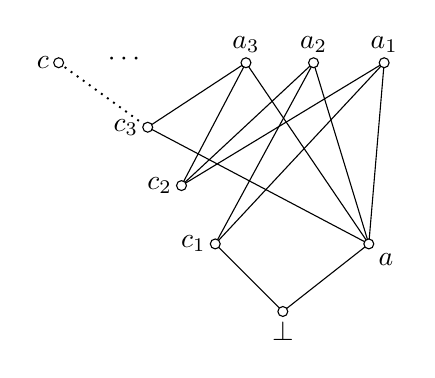
\begin{tikzpicture}[scale=0.78, >=stealth]
  \coordinate (bot) at (3.5,-1.9);
  \coordinate (c1) at (2.4,-0.8);
  \coordinate (c2) at (1.85,0.15);
  \coordinate (c3) at (1.3,1.1);
  \coordinate (a)  at (4.9,-0.8);
  \coordinate (a3) at (2.9,2.15);
  \coordinate (a2) at (4.0,2.15);
  \coordinate (a1) at (5.15,2.15);
  \coordinate (c)  at (-0.15,2.15);
  \foreach \u/\v in {bot/c1,bot/a,c1/a2,c2/a2,c2/a3,c3/a3,c1/a1,c2/a1,c3/a,a/a1,a/a2,a/a3} {
    \draw (\u) -- (\v);
  }
  \draw[dotted, line width=0.7pt] (c) -- (c3);
  \node[left] at (c) {$c$};
  \node[left] at (c3) {$c_3$};
  \node[left] at (c2) {$c_2$};
  \node[left] at (c1) {$c_1$};
  \node[below right] at (a) {$a$};
  \node[above] at (a3) {$a_3$};
  \node[above] at (a2) {$a_2$};
  \node[above] at (a1) {$a_1$};
  \node[below] at (bot) {$\bot$};
  \node at (0.95,2.2) {$\cdots$};
  \foreach \p in {bot,c1,c2,c3,a,a1,a2,a3,c} {
    \filldraw[fill=white] (\p) circle (2.3pt);
  }
\end{tikzpicture}
\par\smallskip\textbf{Figure 13:} An algebraic domain in which topological Egli--Milner ordering and ordinary Egli--Milner ordering do not coincide.
\end{center}

\sourcepage{102}
\leanmarker{lemma-6-2-20}{Lemma 6.2.20} If \(L\) is a Lawson-compact subset of a continuous domain \(D\), then \(\downarrow L\) is Scott-closed.

\leanmarker{cor-6-2-21}{Corollary 6.2.21} In a coherent domain, the lenses are precisely the convex Lawson-compact subsets. For these, topological Egli-Milner ordering and ordinary Egli-Milner ordering coincide.

\leanmarker{thm-6-2-22}{Theorem 6.2.22} If \(D\) is coherent, then the Plotkin powerdomain of \(D\) is isomorphic to
\[
  \langle\operatorname{Lens}(D),\sqsubseteq_{EM}\rangle.
\]
Formal union is interpreted as union followed by convex closure.

\begin{center}
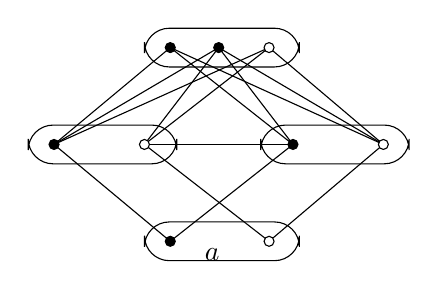
\begin{tikzpicture}[scale=0.82, >=stealth]
  \draw[rounded corners=9pt] (-1.15,1.85) rectangle (1.25,2.45);
  \draw[rounded corners=9pt] (-2.95,0.35) rectangle (-0.65,0.95);
  \draw[rounded corners=9pt] (0.65,0.35) rectangle (2.95,0.95);
  \draw[rounded corners=9pt] (-1.15,-1.15) rectangle (1.25,-0.55);
  \coordinate (t1) at (-0.75,2.15); \coordinate (t2) at (0,2.15); \coordinate (t3) at (0.78,2.15);
  \coordinate (l1) at (-2.55,0.65); \coordinate (l2) at (-1.15,0.65);
  \coordinate (r1) at (1.15,0.65); \coordinate (r2) at (2.55,0.65);
  \coordinate (b1) at (-0.75,-0.85); \coordinate (b2) at (0.78,-0.85);
  \foreach \u/\v in {b1/l1,b1/r1,b2/l2,b2/r2,l1/t1,l1/t2,l2/t2,l2/t3,r1/t1,r1/t2,r2/t2,r2/t3,l2/r1,t1/r2,t3/l1} {
    \draw (\u) -- (\v);
  }
  \foreach \p in {t1,t2,l1,r1,b1} {\filldraw[fill=black] (\p) circle (2.2pt);}
  \foreach \p in {t3,l2,r2,b2} {\filldraw[fill=white] (\p) circle (2.2pt);}
  \node at (-0.1,-1.05) {$a$};
\end{tikzpicture}
\par\smallskip\textbf{Figure 14:} Part of an algebraic domain where Theorem 6.2.19 fails.
\end{center}

\end{document}
